\newpage
\section{Text-to-tree transformation}
\genHeader

Now that our workspace is successfully prepared, let's discuss how the transformation will proceed. For reference, Fig.~\ref{fig:moca-4-Tokens} depicts a small
sample of the textual syntax that will specify a dictionary instance. As we shall see in a moment, the libraries and shelves containing each dictionary correspond to a folder structure, while the
contents for a single dictionary are specified in a file.

\begin{figure}[!htbp]
\begin{center}
 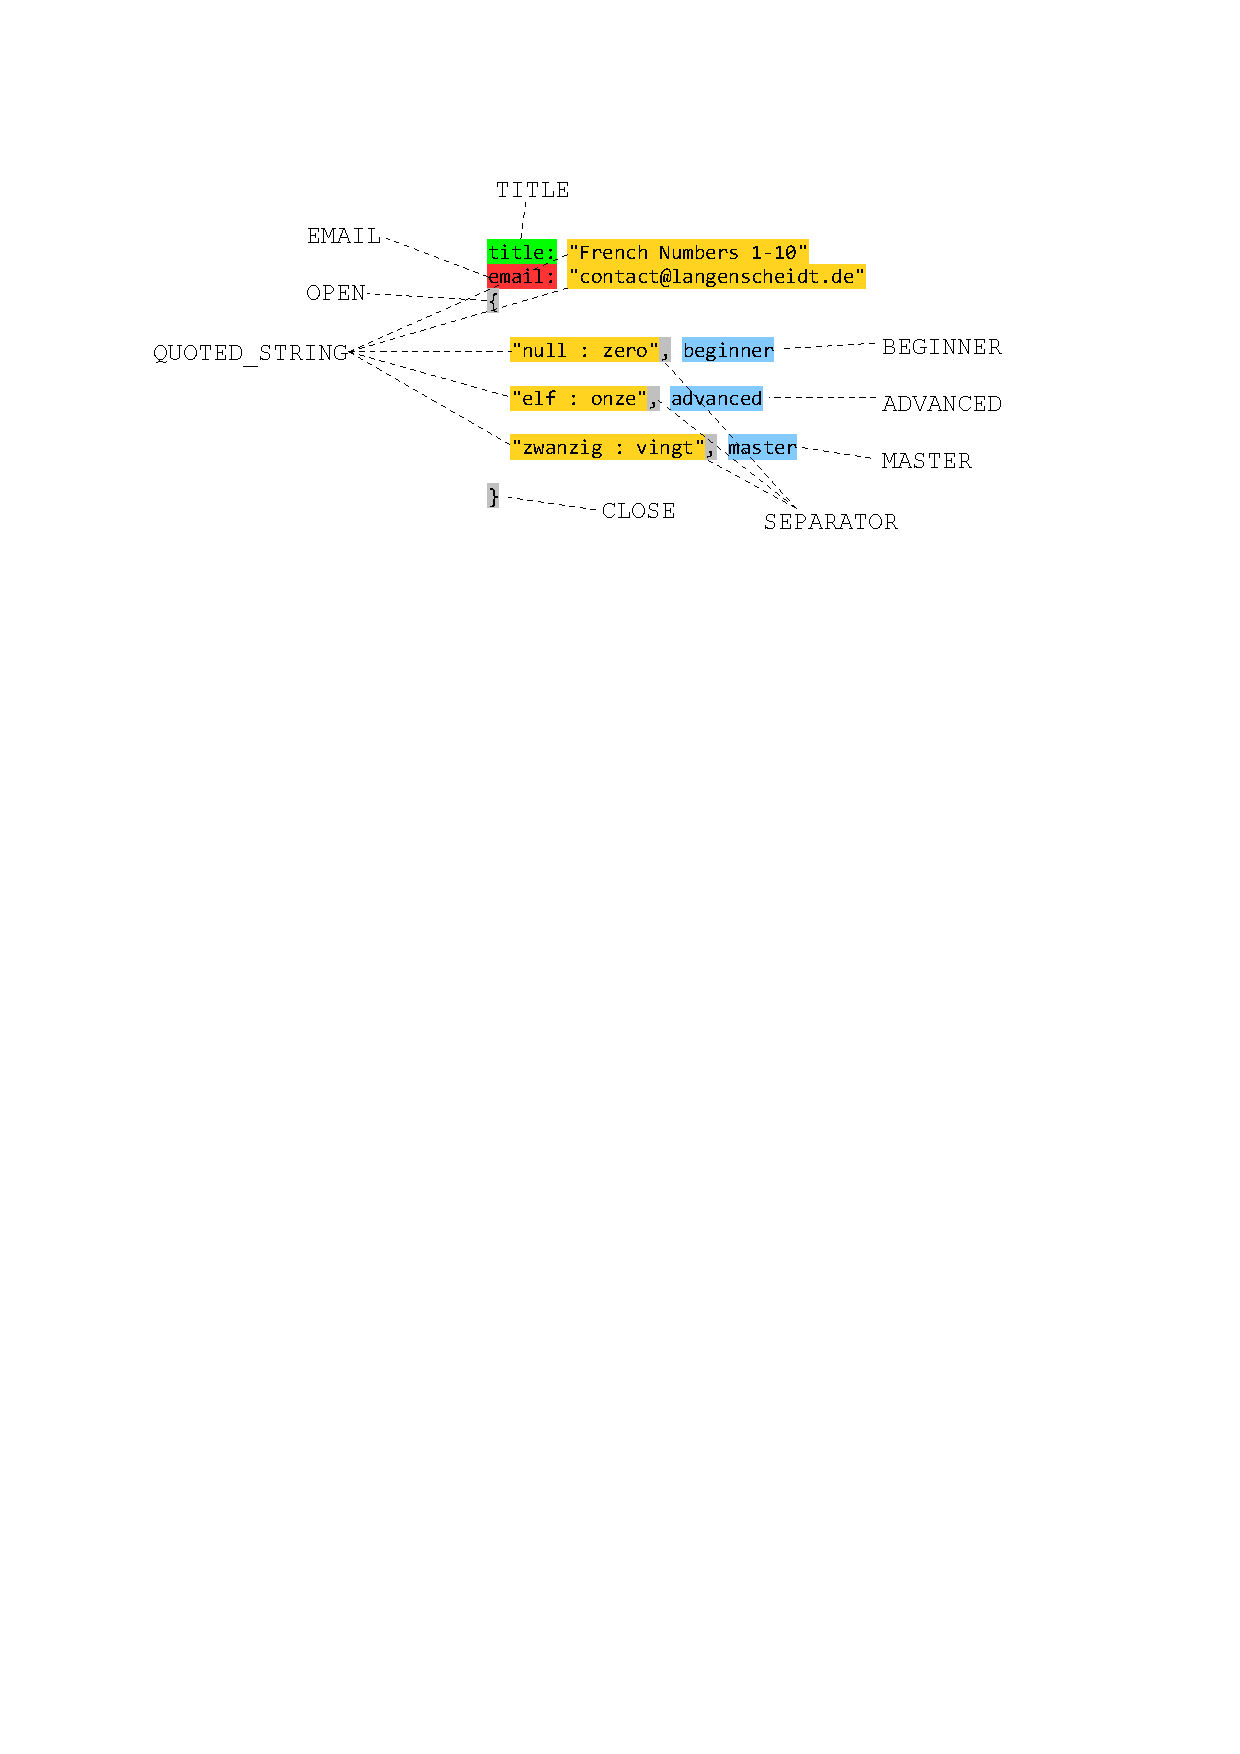
\includegraphics[width=0.7\textwidth]{4-tokens}
  \caption{Identified tokens in a dictionary file}
  \label{fig:moca-4-Tokens}
\end{center}
\end{figure}

On the way to an instance model of our dictionary metamodel, the very first step is to create nice \emph{chunks} of characters. This step is called
\emph{lexing} and it simplifies the comprehension of the complete text. Interestingly, human beings actually comprehend text in a similar manner; one
recognizes whole words without ``seeing'' every individual character. This is the reason why you can siltl raed tihs sneentce alsomt eforftlsesly. A lexer
recognizes these chunks or \emph{tokens} and passes them on as a token stream to the \emph{parser} that does the actual work of recognizing complex
hierarchical and recursive structures.
   
To recognize the tokens as indicated in Fig.~\ref{fig:moca-4-Tokens}, \texttt{ANTLR} can automatically generate a lexer in Java from a compact specification.
This is actually a DSL for lexing and is explained in detail in \cite{ANTLR}. If you are unfamiliar with EBNF, and feel you may have problems understanding
the lexer grammar, we suggest going through the documentation on \url{www.antlr.org}, or reading the relevant chapters in \cite{ANTLR}. Otherwise, let's
complete the \emph{lexer} and \emph{parser} grammars that will handle our project instances.

\begin{itemize}
  
\item[$\blacktriangleright$] Navigate to ``Diction\-ary\-Code\-Adap\-ter/src/org.moflon.moca.dict\-ion\-ary\-.pars\-er" and edit \texttt{DictionaryLexer.g}
until it matches Fig.~\ref{eclipse:dictionaryLexer}. 


\newpage

\begin{figure}[!htbp]
\begin{center}
  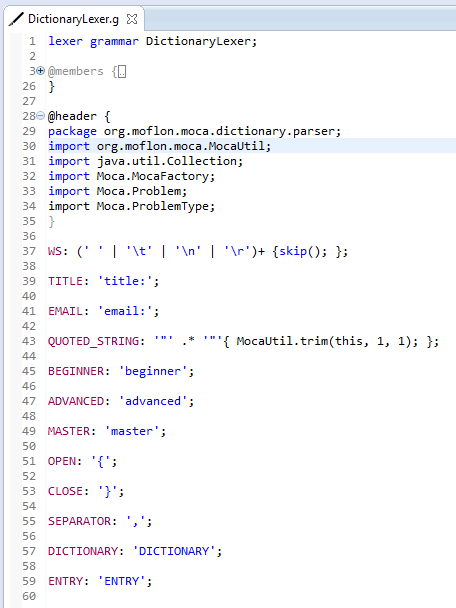
\includegraphics[width=0.7\textwidth]{eclipse_dictionaryLexer}
  \caption{Lexer grammar}
  \label{eclipse:dictionaryLexer}
\end{center}
\end{figure}

\item[$\blacktriangleright$] Don't forget to add \texttt{import org.moflon.moca.MocaUtil} to \texttt{@header}. Be vigilant to avoid any typos and mistakes!

\vspace{0.5cm}

\item[$\blacktriangleright$] Save to compile the file, and ensure no errors persist before proceeding.

\end{itemize}

\vspace{0.25cm}

To briefly explain the two complicated-looking rules, note that the \texttt{WS} rule simply ignores white space. The \texttt{`skip()'} statement throws away the
tokens matched as white space each time they're found in a stream. Similarly, \texttt{QUOTED\_STRING} calls \texttt{`MocaUtil.trim(\ldots)'}, which trims a
recognized token by removing the specified number of characters at its beginning and end. In this case, the token is everything between the `\texttt{''}'
characters, as indicated by the \texttt{`.*'} symbol.

\newpage

Now let's establish a parser to form a file's stream of tokens (as created by the lexer) into a \emph{tree}. In this context, a tree is an acyclic,
hierarchical, recursive structure as depicted in Fig.~\ref{fig:dictLexer}. Depending on what the tree is to be used for, it can be organized differently
using extra \emph{structural} nodes such as \texttt{DICTIONARY} or \texttt{ENTRY} which were not present in the textual syntax. These can be used to give
additional semantics to the tree.

\vspace{0.5cm}

\begin{figure}[htp]
\begin{center}
 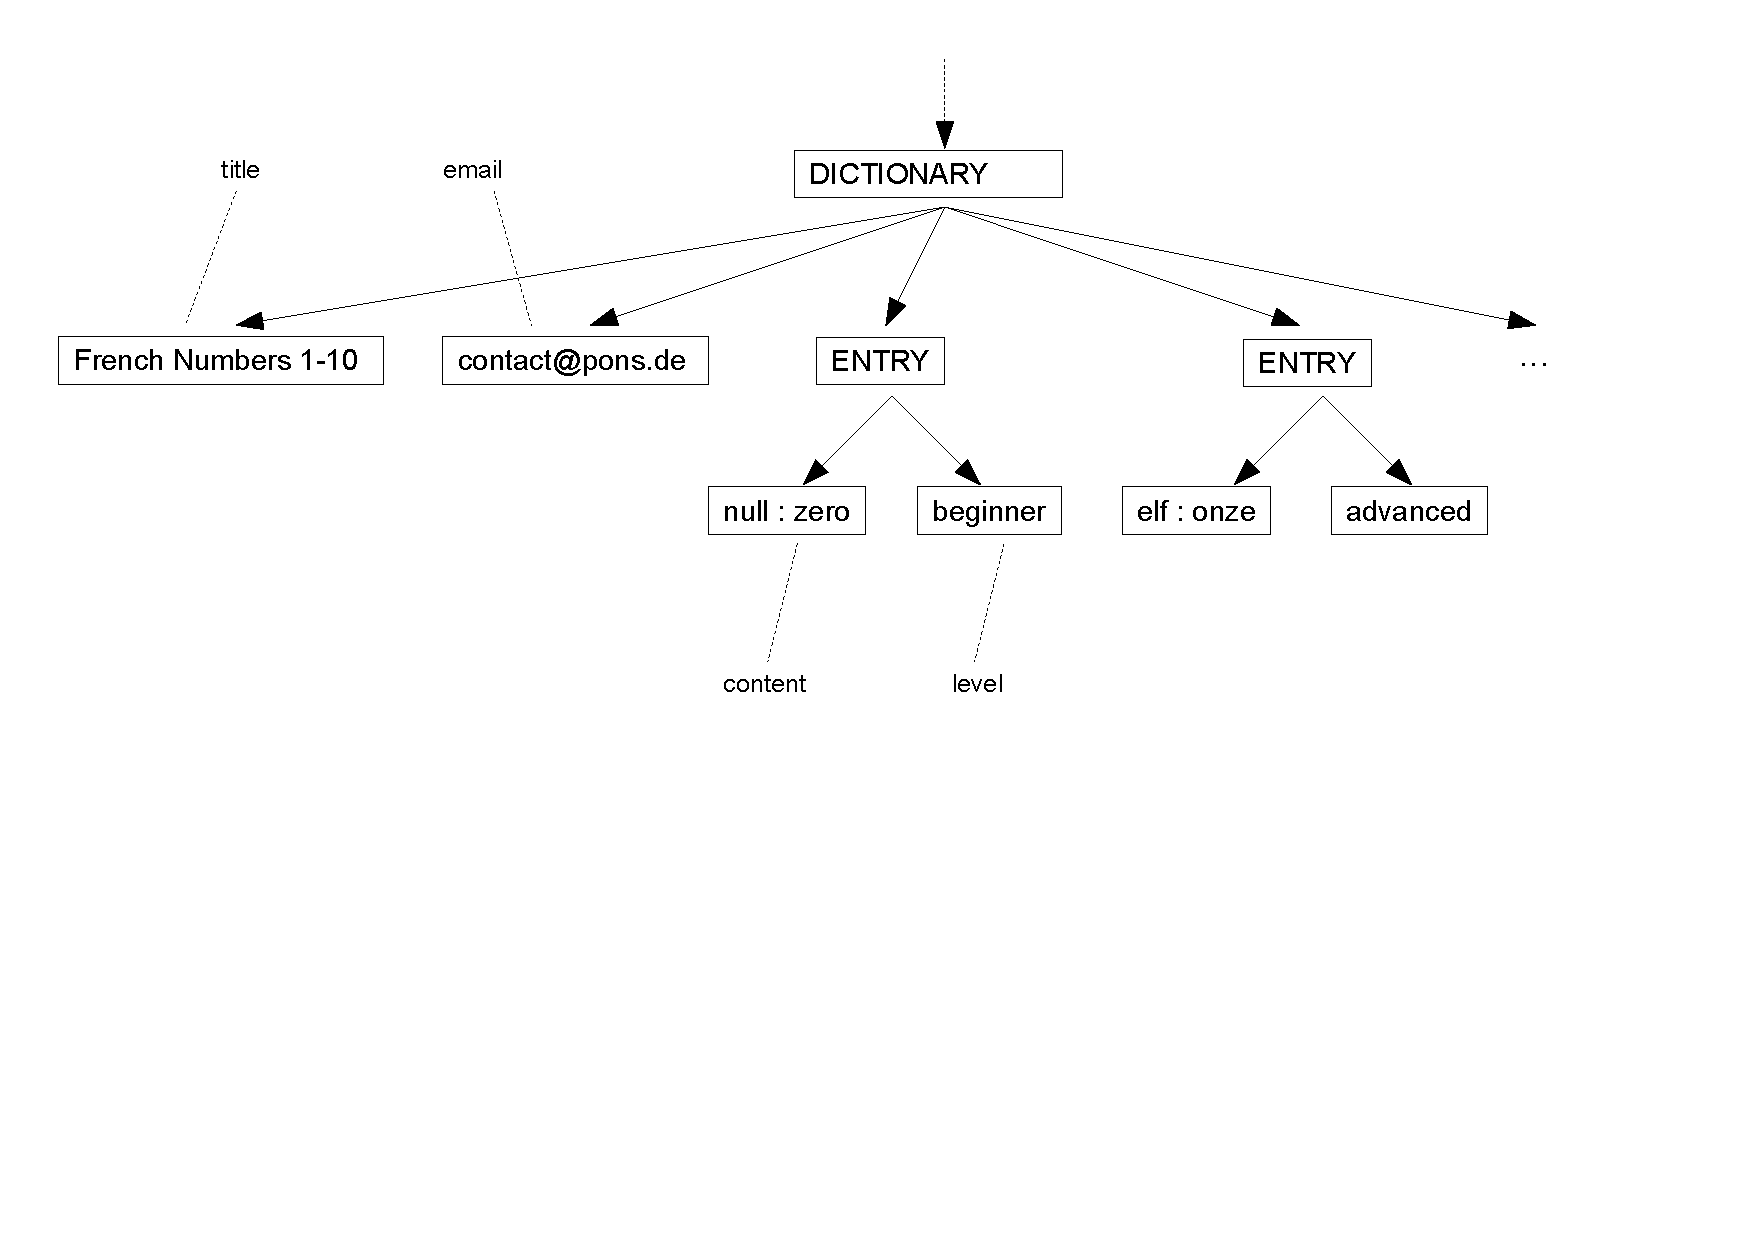
\includegraphics[width=\textwidth]{5-tree}
  \caption{Abstract Syntax Tree (AST) of an input token stream}
  \label{fig:dictLexer}
\end{center}
\end{figure}

\begin{itemize}

\item[$\blacktriangleright$] From the same package, open and edit \texttt{DictionaryParser.g} until it matches Fig.~\ref{eclipse:dictParser}. As with the lexer,
avoid any mistakes, and ensure it compiles before proceeding.

\end{itemize}

\begin{figure}[!htbp]
\begin{center}
 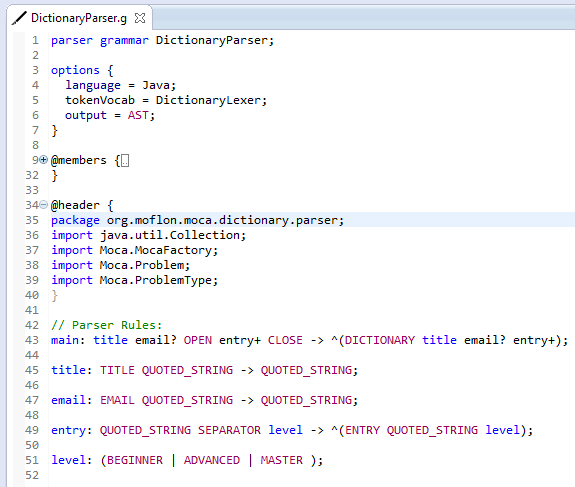
\includegraphics[width=0.9\textwidth]{eclipse_dictionaryParser}
  \caption{Parser grammar}
  \label{eclipse:dictParser}
\end{center}
\end{figure}

You'll notice that the parser grammar is extremely similar to the lexer grammar, save for some \emph{parser actions} following the \texttt{`->'} symbol. These
actions control the construction of the resulting tree. Using this simple tree language, one can (1) abstract from tokens such as \texttt{`\{'} or
\texttt{`\}'}, which are just \emph{syntactical noise}\footnote{Irrelevant content for our model} and (2) enrich the tree with structural nodes such as
\texttt{ENTRY}, which add explicit structure to the tree. Refer to \cite{ANTLR} and online resources for detailed explanations on the syntax and semantics of
the parser grammar supported by \texttt{ANTLR}.

\newpage

\begin{itemize}

\item[$\blacktriangleright$] Before taking our lexer and parser for a spin, navigate to ``src\-/org\-.mof\-lon\-.tie" and open
\texttt{DictionaryCodeAdapterTrafo.java}. We need to update the file so that it will work with our specific project, so add the highlighted areas in
Fig.~\ref{eclipse:defaultTGGMain} to the file.

\vspace{0.5cm}

\begin{figure}[!htbp]
\begin{center}
 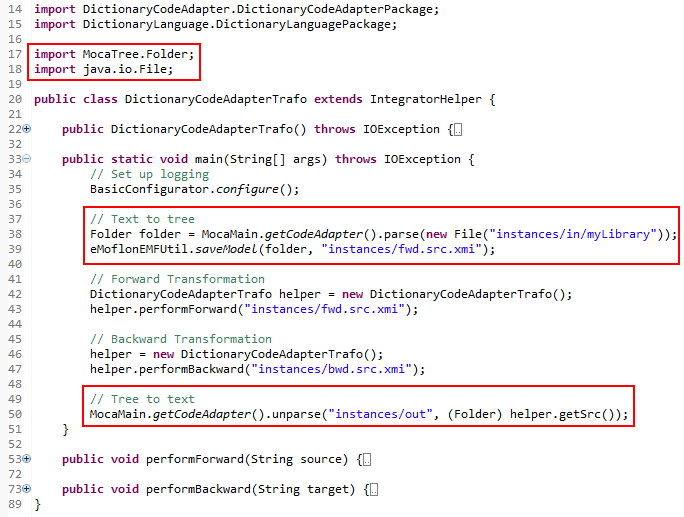
\includegraphics[width=\textwidth]{eclipse_editTrafo}
  \caption{Edit \texttt{DictionaryCodeAdapterTrafo} to run the transformation}
  \label{eclipse:defaultTGGMain}
\end{center}
\end{figure}

\end{itemize}

You can see that this main method is essentially the driver for a complete transformation, executing four stages for a forward and backward transform. In a
nutshell, each folder in ``instances/in/myLibrary'' is taken as the root of a tree, and their folder and file structures will be reflected as a hierarchy of
(children) nodes in the tree. For each file, the framework will search for a registered parser that is responsible for the particular file, pass the content
onto the parser, then plug in the tree generated from the parser as a single subtree of the corresponding file node in the overall tree.

In this example, the framework uses our parser on \texttt{.dictionary} files, the file extension we specified when creating the lexer and parser stubs
(Fig.~\ref{eclipse:generatedParser}). Of course, this method (in the generated \texttt{parserAdapter}) can be overridden to register e.g., multiple
file extensions, or peek into the actual file content and base its parsing decision on what it finds.

\begin{itemize}

\item[$\blacktriangleright$] To prepare some input for the framework, navigate to ``Dict\-ion\-ar\-y\-Code\-Adap\-ter\-/in\-stan\-ces\-/in'' and create the
filesystem depicted in \\ Fig.~\ref{eclipse:textDirectory}. 

\begin{figure}[htp]
\begin{center}
  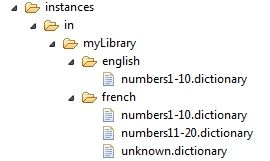
\includegraphics[width=0.5\textwidth]{inputData}
  \caption{Input directory structure}
  \label{eclipse:textDirectory}
\end{center}
\end{figure}

\item[$\blacktriangleright$] Complete each of the four \texttt{.dictionary} files with the contents in Table~\ref{moca-inputdata}.\footnote{If you copy and
paste this data, be careful as your .pdf reader may add some invisible characters to the file that ANTLR will not detect and ignore as white space.} 
Be vigilant to ensure there are no mistakes with symbols such as colons or commas!

\end{itemize}

As you can see, the input folder is structured as a single library, \texttt{myLibrary}, and split into two languages, english and french, each containing
some dictionaries. Reviewing Fig.~\ref{eclipse:dictParser}, you can see that the structure of these files conforms to the parser's \texttt{main} rule: it
first lists the dictionary's \texttt{title}, may or may not contain an \texttt{author}, and contains all \texttt{entry} elements between a pair of \texttt{OPEN}
and \texttt{CLOSE} brackets.

\newpage
\begin{table}

\begin{tabular}{p{6cm} p{6cm} }
\footnotesize
\textbf{english/numbers1-10.dictionary:}
\begin{verbatim}
title: "numbers1-10"
email: "contact@langenscheidt.de"	
{
  "null : zero", beginner
  "eins : one", beginner
  "zwei : two", beginner
  "drei : three", beginner
  "vier : four", beginner
  "fuenf : five", beginner
  "sechs : six", beginner
  "sieben : seven", beginner
  "acht : eight", beginner
  "neun : nine", beginner
  "zehn : ten", beginner 
}
\end{verbatim} 

\vspace{0.5cm}

\footnotesize
\textbf{french/numbers11-20.dictionary:}
\begin{verbatim}
title: "numbers11-20"
email: "contact@pons.de"	
{
  "elf : onze", advanced
  "zwoelf : douze", advanced
  "dreizehn : treize", advanced
  "vierzehn : quatorze", advanced
  "fuenfzehn : quinze", advanced
  "sechzehn : seize", master
  "siebzehn : dix-sept", master
  "achtzehn : dix-huit", master
  "neunzehn : dix-neuf", master
  "zwanzig : vingt", master
}
\end{verbatim}
&

\footnotesize
\textbf{french/numbers1-10.dictionary:}
\begin{verbatim}   
title: "numbers1-10"
email: "contact@pons.de"	
{
  "null : zero", beginner
  "eins : un/une", beginner
  "zwei : deux", beginner
  "drei : trois", beginner
  "vier : quatre", beginner
  "fuenf : cinq", beginner
  "sechs : six", beginner
  "sieben : sept", beginner
  "acht : huit", beginner
  "neun : neuf", beginner
  "zehn : dix", beginner 
}
\end{verbatim}

\vspace{0.5cm}

\footnotesize
\textbf{french/unknown.dictionary:}
\begin{verbatim}
title: "unknown"
{
	"unbekannt : unknown", beginner
}
\end{verbatim}
  \\
\end{tabular}   
\caption{Four input \texttt{.dictionary} files}
\label{moca-inputdata}

\end{table}
\clearpage

\begin{itemize} 

\item[$\blacktriangleright$] Once you have saved each file, right click on \texttt{Dict\-ion\-ar\-y\-Code\-Ad\-ap\-ter\-Traf\-o.\-java} and navigate to ``Run
As/Java Application'' to run the transformation. Don't worry about the error messages -- they're related to the unparser which we haven't implemented yet; You
should have received at least one success message indicating your transformation worked.

\item[$\blacktriangleright$] Refresh the \texttt{instances} folder. Despite being (mostly) unimplemented, the transformation still partly completed, generating
several files in the process (Fig.~\ref{eclipse:postParse}).

\vspace{0.5cm}

\begin{figure}[!htbp]
\begin{center}
 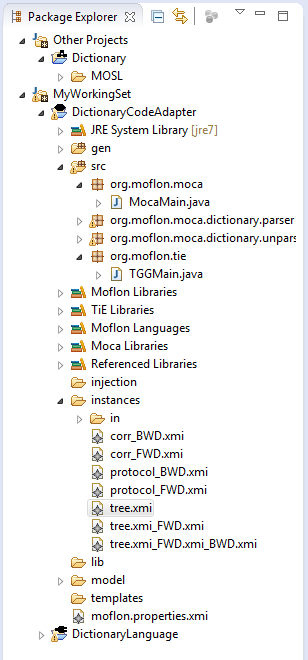
\includegraphics[width=0.5\textwidth]{eclipse_explorerPostGeneration}
  \caption{Result of the first TGG execution}
  \label{eclipse:postParse}
\end{center}
\end{figure} 

\end{itemize}

Let's go over what each of these files are. First, \texttt{fwd.src.xmi} is the direct result of the \texttt{my\-Lib\-rary} filesystem input, which was parsed
into a \texttt{MocaTree} instance by our ANTLR parser. 

While the parser is the only implemented piece of our transformation, TGGMain still used \texttt{fwd.src.xmi} in a forward transform, producing
the correspondence model \texttt{fwd.corr.xmi} (paired with \texttt{fwd.protocol.xmi}), and the (currently empty) \texttt{Dictionary} target result,
\texttt{fwd.trg.xmi}.

\clearpage

%The TGG also executed in the inverse direction; \texttt{tree.xmi\_FWD.xmi} was used in the backwards direction, producing \texttt{corrBWD.xmi} (with
%\texttt{proto\-col\-\_BWD\-.xmi}) and \texttt{tree.xmi\_FWD.xmi\_BWD.xmi}. 

\begin{itemize}

\item[$\blacktriangleright$] Open \texttt{fwd.src.xmi} and compare the contents to Fig.~\ref{eclipse:treeResult}. Reflect on the directory-type structure of the
tree, where each \texttt{File} and its contents appear as \texttt{Node}s.\footnote{Refer to Fig~\ref{mocaTreeMetamodel} for the metamodel of this structure}
This file is important to understand -- The filesystem was transformed into a corresponding hierarchy of \texttt{Folders} and \texttt{Files}. The actual
\emph{text} content of each file is then transformed to a subtree using a registered, suitable parser. The resulting subtree from the parser is then connected
to the existing tree by setting its \texttt{DICTIONARY} root as the single child node of a \texttt{File}.

\end{itemize}

\vspace{0.5cm}

\begin{figure}[!htbp]
\begin{center}
 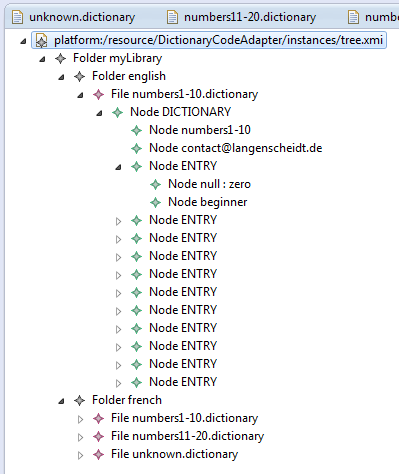
\includegraphics[width=0.6\textwidth]{eclipse_textParsingGeneration}
  \caption{A \texttt{MocaTree} created by the framework using our parser}
  \label{eclipse:treeResult}
\end{center}
\end{figure}

If everything executed without errors, well done! Let's continue with the transformation to a \texttt{Dictionary} instance by specifiying some
TGG rules.
